% !TeX spellcheck = cs_CZ
%{\tikzset{external/prefix={tikz/FYZII/}}
% \tikzset{external/figure name/.add={ch15_}{}}
%---------------------------------------------------------------------------------------------------
% file fey2ch15.tex
%---------------------------------------------------------------------------------------------------
%=========================== Kapitola: Vektorový potenciál =========================================
\chapter{Vektorový potenciál}\label{fyz:IIchaXV}
\minitoc
  \section{Síly působící na proudovou smyčku. Energie dipólu}\label{fyz:IIchaXVsecI}
  \section{Mechanická a elektrická energie}\label{fyz:IIchaXVsecII}
  \section{Energie ustálených proudů}\label{fyz:IIchaXVsecIII}
  \section{B nebo A}\label{fyz:IIchaXVsecIV}
  \section{Vektorový potenciál a kvantová mechanika}\label{fyz:IIchaXVsecV}
  \section{Co platí ve statice neplatí v dynamice}\label{fyz:IIchaXVsecVI}
  \section{Příklady a cvičení}\label{fyz:IIchaXVsecVII}

    \begin{figure}[ht!] %\ref{fyz_fig663}
      \centering
      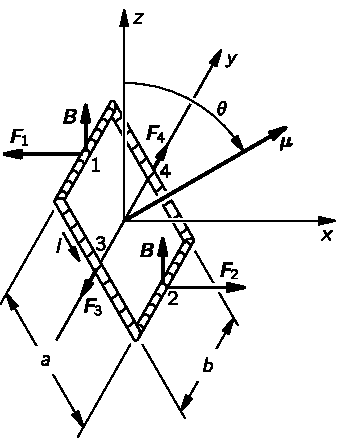
\includegraphics[width=0.7\linewidth]{fyz_fig663.pdf}
      \caption{
               (\cite[s.~707]{Feynman02})}
      \label{fyz_fig663}
    \end{figure}

    \begin{figure}[ht!] %\ref{fyz_fig664}
      \centering
      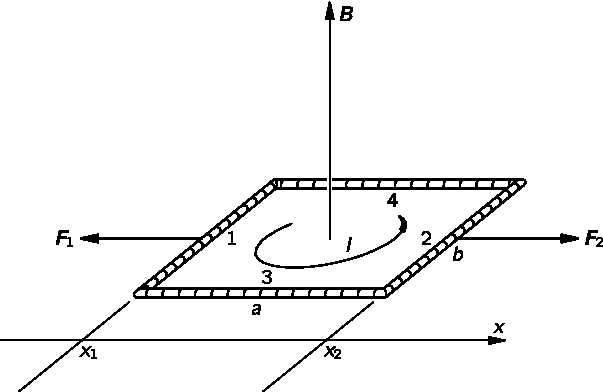
\includegraphics[width=0.7\linewidth]{fyz_fig664.pdf}
      \caption{
               (\cite[s.~707]{Feynman02})}
      \label{fyz_fig664}
    \end{figure}

    \begin{figure}[ht!]
      \centering
      \begin{tabular}{c}
        \subfloat[ ]{\label{fyz_fig665a}
          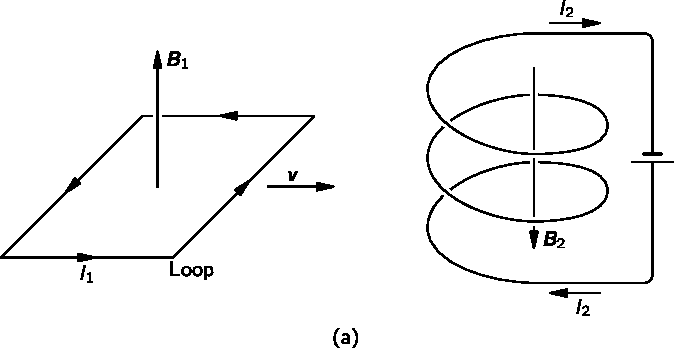
\includegraphics[width=0.7\linewidth]{fyz_fig665a.pdf}}               \\
        \subfloat[ ]{\label{fyz_fig665b}
          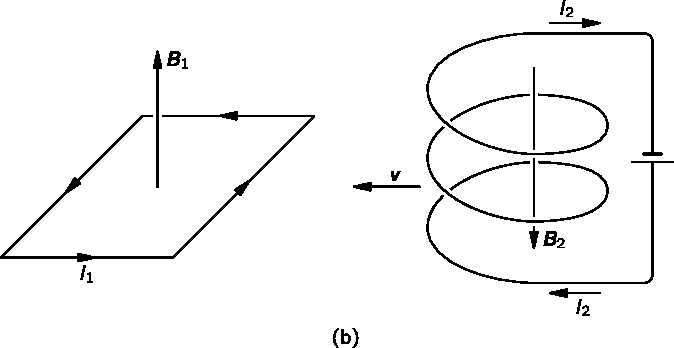
\includegraphics[width=0.7\linewidth]{fyz_fig665b.pdf}}
      \end{tabular}
      \label{fyz_fig665}
      \caption{
               (\cite[s.~748]{Feynman02})}
    \end{figure}

    \begin{figure}[ht!] %\ref{fyz_fig666}
      \centering
      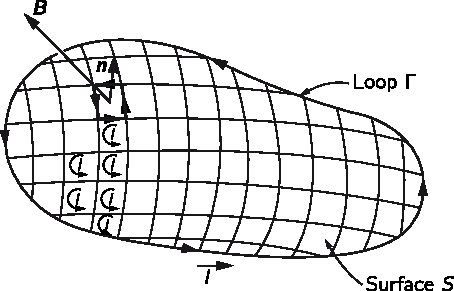
\includegraphics[width=0.7\linewidth]{fyz_fig666.pdf}
      \caption{
               (\cite[s.~707]{Feynman02})}
      \label{fyz_fig666}
    \end{figure}

    \begin{figure}[ht!] %\ref{fyz_fig667}
      \centering
      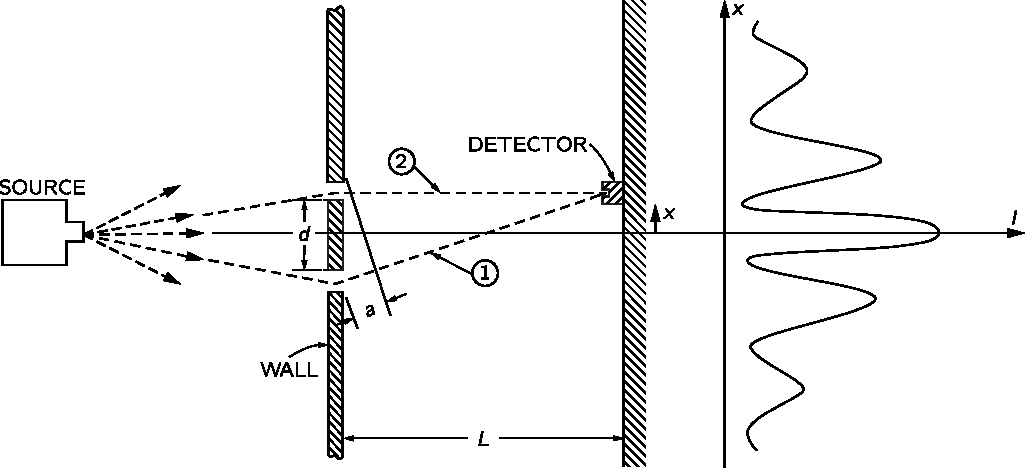
\includegraphics[width=0.7\linewidth]{fyz_fig667.pdf}
      \caption{
               (\cite[s.~707]{Feynman02})}
      \label{fyz_fig667}
    \end{figure}


    \begin{figure}[ht!] %\ref{fyz_fig668}
      \centering
      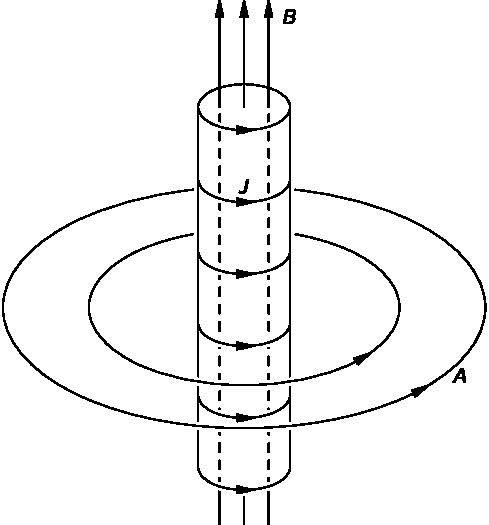
\includegraphics[width=0.7\linewidth]{fyz_fig668.pdf}
      \caption{
               (\cite[s.~707]{Feynman02})}
      \label{fyz_fig668}
    \end{figure}

    \begin{figure}[ht!] %\ref{fyz_fig669}
      \centering
      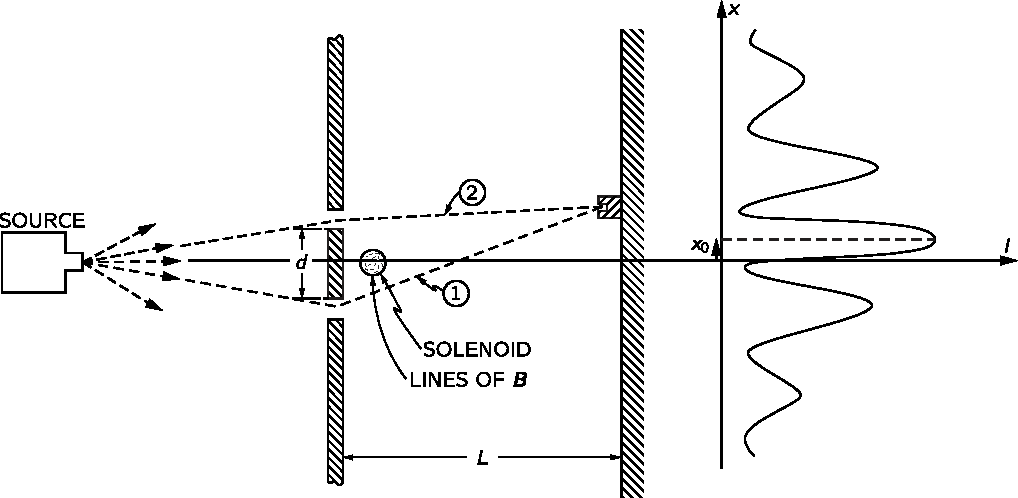
\includegraphics[width=0.7\linewidth]{fyz_fig669.pdf}
      \caption{
               (\cite[s.~707]{Feynman02})}
      \label{fyz_fig669}
    \end{figure}

    \begin{figure}[ht!] %\ref{fyz_fig670}
      \centering
      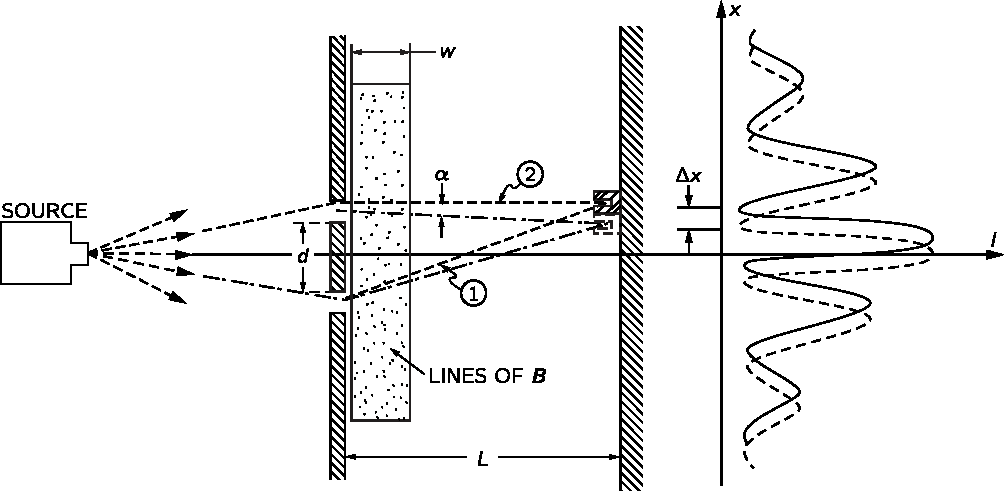
\includegraphics[width=0.7\linewidth]{fyz_fig670.pdf}
      \caption{
               (\cite[s.~707]{Feynman02})}
      \label{fyz_fig670}
    \end{figure}


    \begin{figure}[ht!] %\ref{fyz_fig671}
      \centering
      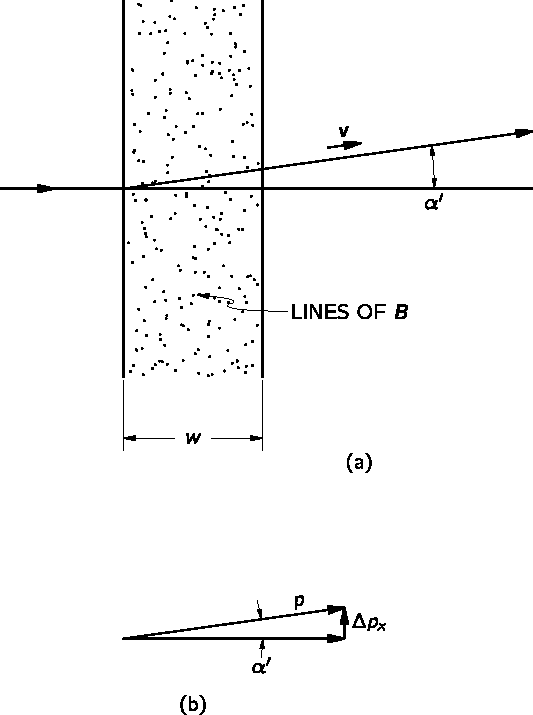
\includegraphics[width=0.7\linewidth]{fyz_fig671.pdf}
      \caption{
               (\cite[s.~707]{Feynman02})}
      \label{fyz_fig671}
    \end{figure}

    \begin{figure}[ht!] %\ref{fyz_fig672}
      \centering
      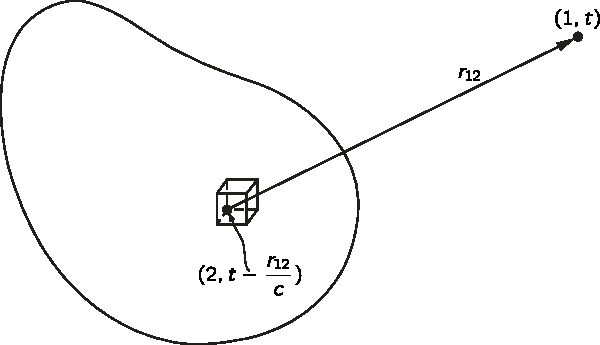
\includegraphics[width=0.7\linewidth]{fyz_fig672.pdf}
      \caption{
               (\cite[s.~707]{Feynman02})}
      \label{fyz_fig672}
    \end{figure}

%} %tikzset
%---------------------------------------------------------------------------------------------------
\printbibliography[title={Seznam literatury},heading=subbibliography]
\addcontentsline{toc}{section}{Seznam literatury}